
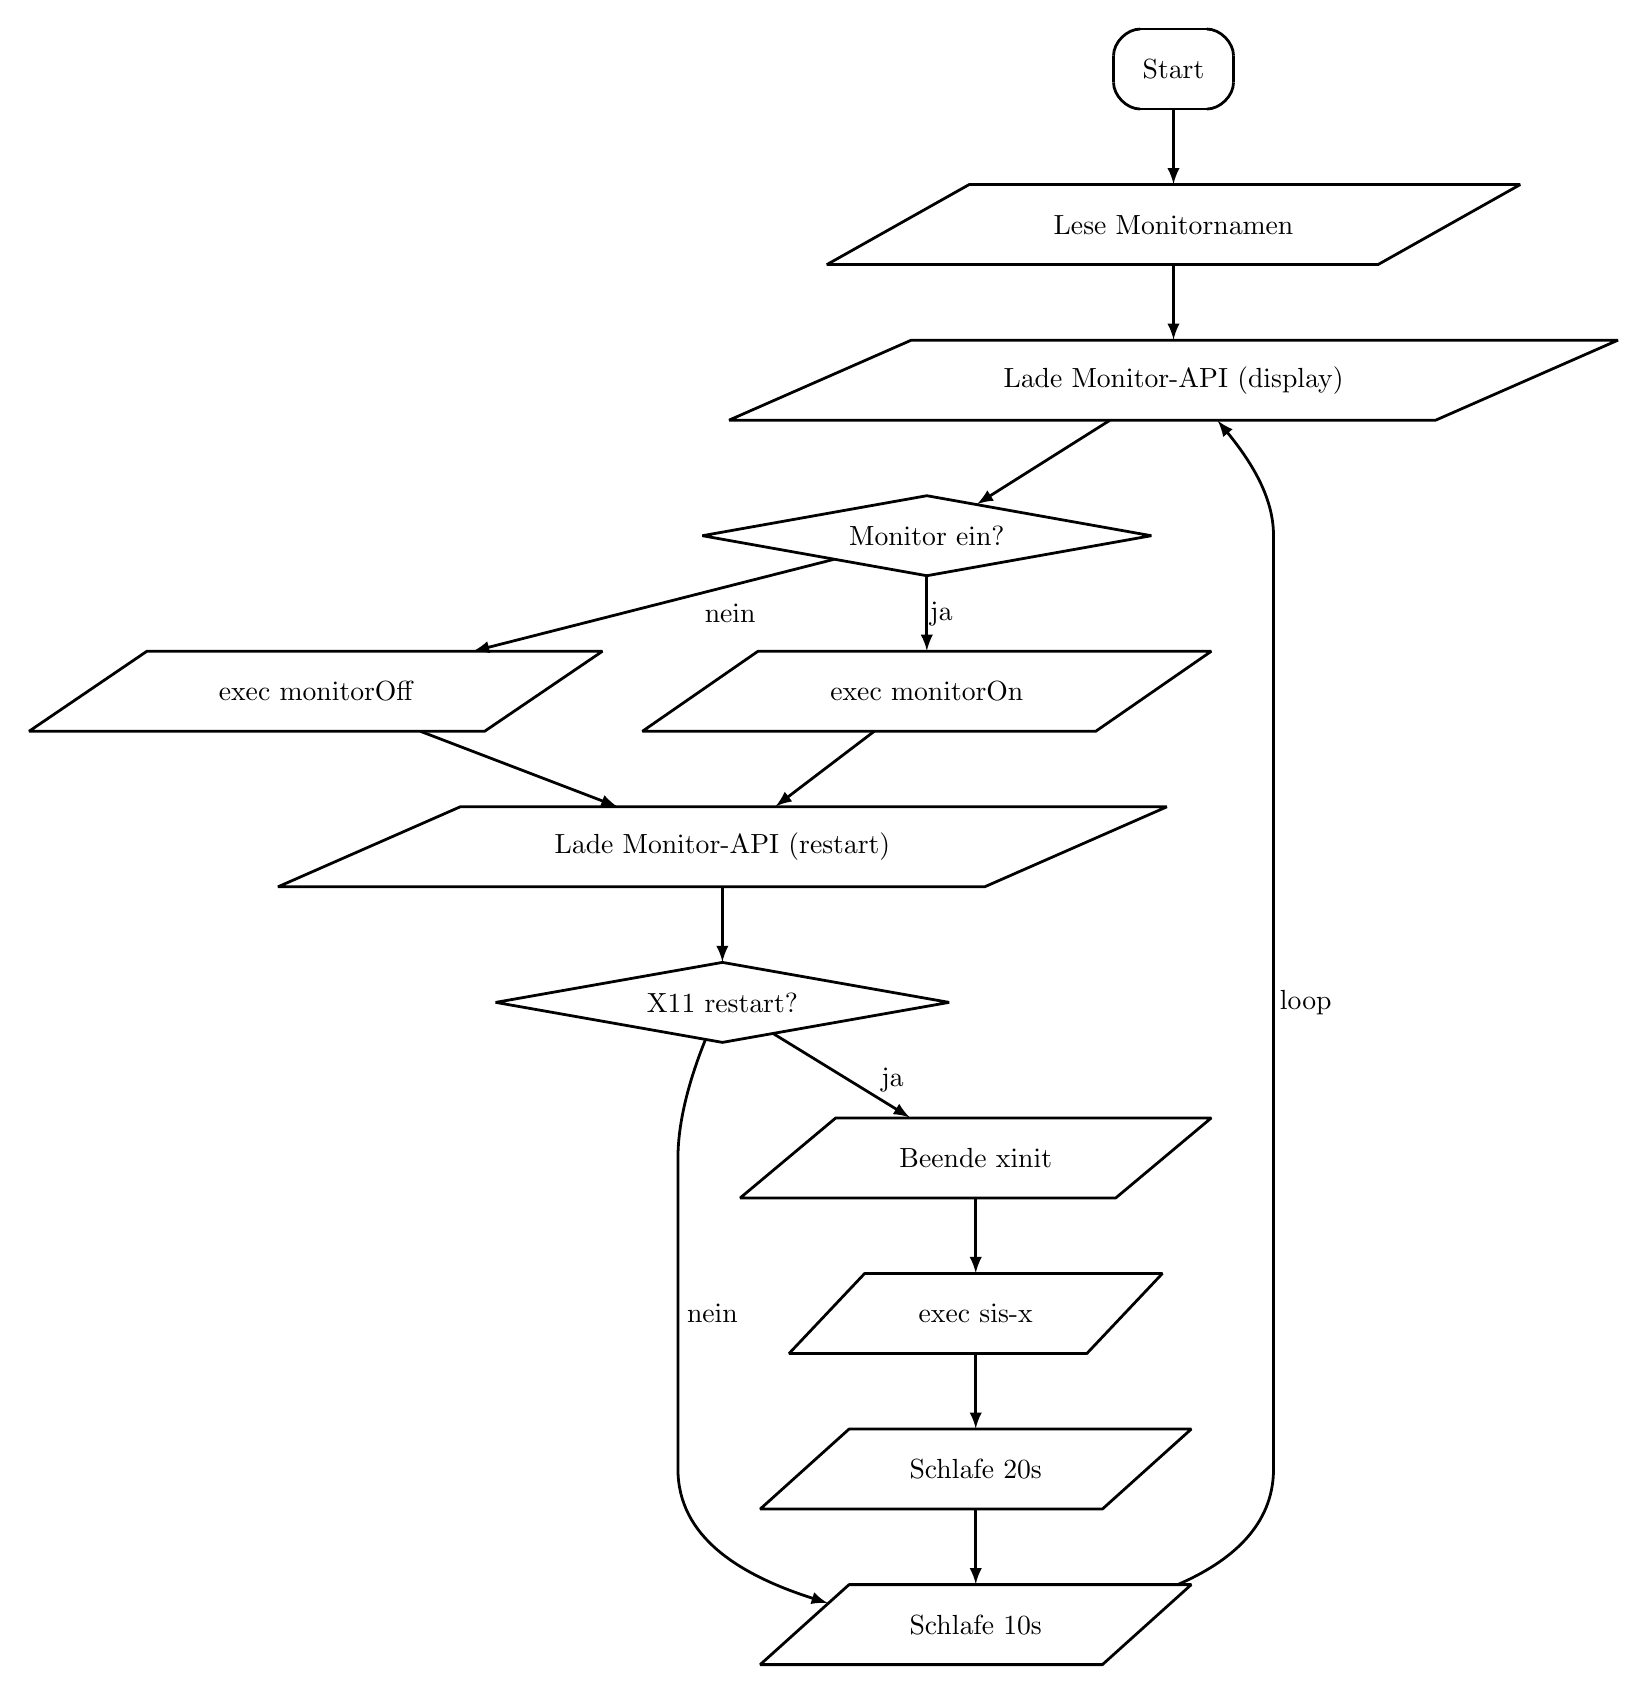
\begin{tikzpicture}[>=latex,line join=bevel,scale=0.8]
  \pgfsetlinewidth{1bp}
%%
\pgfsetcolor{black}
  % Edge: X11 restart? -> Schlafe 10s
  \draw [->] (304.32bp,281.12bp) .. controls (298.68bp,267.18bp) and (292bp,246.71bp)  .. (292bp,228bp) .. controls (292bp,228bp) and (292bp,228bp)  .. (292bp,88bp) .. controls (292bp,57.566bp) and (319.49bp,40.341bp)  .. (359.39bp,27.697bp);
  \definecolor{strokecol}{rgb}{0.0,0.0,0.0};
  \pgfsetstrokecolor{strokecol}
  \draw (307.5bp,158bp) node {nein};
  % Edge: Schlafe 10s -> Lade Monitor-API (display)
  \draw [->] (516.86bp,36.003bp) .. controls (540.76bp,46.325bp) and (560bp,62.541bp)  .. (560bp,88bp) .. controls (560bp,508bp) and (560bp,508bp)  .. (560bp,508bp) .. controls (560bp,524.2bp) and (551.37bp,539.64bp)  .. (534.87bp,559.8bp);
  \draw (574.5bp,298bp) node {loop};
  % Edge: Schlafe 20s -> Schlafe 10s
  \draw [->] (426bp,69.973bp) .. controls (426bp,62.763bp) and (426bp,54.284bp)  .. (426bp,36.209bp);
  % Edge: exec monitorOn -> Lade Monitor-API (restart)
  \draw [->] (380.31bp,419.97bp) .. controls (369.23bp,411.55bp) and (355.88bp,401.39bp)  .. (335.93bp,386.21bp);
  % Edge: Beende xinit -> exec sis-x
  \draw [->] (426bp,209.97bp) .. controls (426bp,202.76bp) and (426bp,194.28bp)  .. (426bp,176.21bp);
  % Edge: Lese Monitornamen -> Lade Monitor-API (display)
  \draw [->] (515bp,629.97bp) .. controls (515bp,622.76bp) and (515bp,614.28bp)  .. (515bp,596.21bp);
  % Edge: Start -> Lese Monitornamen
  \draw [->] (515bp,699.97bp) .. controls (515bp,692.76bp) and (515bp,684.28bp)  .. (515bp,666.21bp);
  % Edge: Monitor ein? -> exec monitorOn
  \draw [->] (404bp,489.97bp) .. controls (404bp,482.76bp) and (404bp,474.28bp)  .. (404bp,456.21bp);
  \draw (410.5bp,473bp) node {ja};
  % Edge: Monitor ein? -> exec monitorOff
  \draw [->] (362.23bp,497.37bp) .. controls (321.88bp,487.1bp) and (259.67bp,471.26bp)  .. (199.82bp,456.03bp);
  \draw (315.5bp,473bp) node {nein};
  % Edge: exec sis-x -> Schlafe 20s
  \draw [->] (426bp,139.97bp) .. controls (426bp,132.76bp) and (426bp,124.28bp)  .. (426bp,106.21bp);
  % Edge: Lade Monitor-API (restart) -> X11 restart?
  \draw [->] (312bp,349.97bp) .. controls (312bp,342.76bp) and (312bp,334.28bp)  .. (312bp,316.21bp);
  % Edge: Lade Monitor-API (display) -> Monitor ein?
  \draw [->] (486.41bp,559.97bp) .. controls (470.7bp,550.06bp) and (451.18bp,537.75bp)  .. (426.54bp,522.21bp);
  % Edge: X11 restart? -> Beende xinit
  \draw [->] (334.8bp,284bp) .. controls (349.85bp,274.76bp) and (369.94bp,262.42bp)  .. (396.32bp,246.23bp);
  \draw (388.5bp,263bp) node {ja};
  % Edge: exec monitorOff -> Lade Monitor-API (restart)
  \draw [->] (176.13bp,419.97bp) .. controls (200.26bp,410.74bp) and (229.83bp,399.43bp)  .. (264.71bp,386.09bp);
  % Node: exec monitorOff
\begin{scope}
  \definecolor{strokecol}{rgb}{0.0,0.0,0.0};
  \pgfsetstrokecolor{strokecol}
  \draw (258bp,456bp) -- (53bp,456bp) -- (0bp,420bp) -- (205bp,420bp) -- cycle;
  \draw (129bp,438bp) node {exec monitorOff};
\end{scope}
  % Node: exec monitorOn
\begin{scope}
  \definecolor{strokecol}{rgb}{0.0,0.0,0.0};
  \pgfsetstrokecolor{strokecol}
  \draw (532bp,456bp) -- (328bp,456bp) -- (276bp,420bp) -- (480bp,420bp) -- cycle;
  \draw (404bp,438bp) node {exec monitorOn};
\end{scope}
  % Node: Schlafe 20s
\begin{scope}
  \definecolor{strokecol}{rgb}{0.0,0.0,0.0};
  \pgfsetstrokecolor{strokecol}
  \draw (523bp,106bp) -- (369bp,106bp) -- (329bp,70bp) -- (483bp,70bp) -- cycle;
  \draw (426bp,88bp) node {Schlafe 20s};
\end{scope}
  % Node: Monitor ein?
\begin{scope}
  \definecolor{strokecol}{rgb}{0.0,0.0,0.0};
  \pgfsetstrokecolor{strokecol}
  \draw (404bp,526bp) -- (303bp,508bp) -- (404bp,490bp) -- (505bp,508bp) -- cycle;
  \draw (404bp,508bp) node {Monitor ein?};
\end{scope}
  % Node: X11 restart?
\begin{scope}
  \definecolor{strokecol}{rgb}{0.0,0.0,0.0};
  \pgfsetstrokecolor{strokecol}
  \draw (312bp,316bp) -- (210bp,298bp) -- (312bp,280bp) -- (414bp,298bp) -- cycle;
  \draw (312bp,298bp) node {X11 restart?};
\end{scope}
  % Node: Start
\begin{scope}
  \definecolor{strokecol}{rgb}{0.0,0.0,0.0};
  \pgfsetstrokecolor{strokecol}
  \draw (530bp,736bp) -- (500bp,736bp);
  \draw (500bp,736bp) .. controls (494bp,736bp) and (488bp,730bp)  .. (488bp,724bp);
  \draw (488bp,724bp) -- (488bp,712bp);
  \draw (488bp,712bp) .. controls (488bp,706bp) and (494bp,700bp)  .. (500bp,700bp);
  \draw (500bp,700bp) -- (530bp,700bp);
  \draw (530bp,700bp) .. controls (536bp,700bp) and (542bp,706bp)  .. (542bp,712bp);
  \draw (542bp,712bp) -- (542bp,724bp);
  \draw (542bp,724bp) .. controls (542bp,730bp) and (536bp,736bp)  .. (530bp,736bp);
  \draw (515bp,718bp) node {Start};
\end{scope}
  % Node: Lese Monitornamen
\begin{scope}
  \definecolor{strokecol}{rgb}{0.0,0.0,0.0};
  \pgfsetstrokecolor{strokecol}
  \draw (671bp,666bp) -- (423bp,666bp) -- (359bp,630bp) -- (607bp,630bp) -- cycle;
  \draw (515bp,648bp) node {Lese Monitornamen};
\end{scope}
  % Node: Beende xinit
\begin{scope}
  \definecolor{strokecol}{rgb}{0.0,0.0,0.0};
  \pgfsetstrokecolor{strokecol}
  \draw (532bp,246bp) -- (363bp,246bp) -- (320bp,210bp) -- (489bp,210bp) -- cycle;
  \draw (426bp,228bp) node {Beende xinit};
\end{scope}
  % Node: Lade Monitor-API (display)
\begin{scope}
  \definecolor{strokecol}{rgb}{0.0,0.0,0.0};
  \pgfsetstrokecolor{strokecol}
  \draw (715bp,596bp) -- (397bp,596bp) -- (315bp,560bp) -- (633bp,560bp) -- cycle;
  \draw (515bp,578bp) node {Lade Monitor-API (display)};
\end{scope}
  % Node: Lade Monitor-API (restart)
\begin{scope}
  \definecolor{strokecol}{rgb}{0.0,0.0,0.0};
  \pgfsetstrokecolor{strokecol}
  \draw (512bp,386bp) -- (194bp,386bp) -- (112bp,350bp) -- (430bp,350bp) -- cycle;
  \draw (312bp,368bp) node {Lade Monitor-API (restart)};
\end{scope}
  % Node: Schlafe 10s
\begin{scope}
  \definecolor{strokecol}{rgb}{0.0,0.0,0.0};
  \pgfsetstrokecolor{strokecol}
  \draw (523bp,36bp) -- (369bp,36bp) -- (329bp,0bp) -- (483bp,0bp) -- cycle;
  \draw (426bp,18bp) node {Schlafe 10s};
\end{scope}
  % Node: exec sis-x
\begin{scope}
  \definecolor{strokecol}{rgb}{0.0,0.0,0.0};
  \pgfsetstrokecolor{strokecol}
  \draw (510bp,176bp) -- (376bp,176bp) -- (342bp,140bp) -- (476bp,140bp) -- cycle;
  \draw (426bp,158bp) node {exec sis-x};
\end{scope}
%
\end{tikzpicture}

